% PhyCL-Net Architecture Diagram
% Compile: pdflatex phycl_net_architecture.tex
\documentclass[tikz, border=10pt]{standalone}
\usepackage{tikz}
\usetikzlibrary{shapes.geometric, arrows.meta, positioning, fit, calc, backgrounds, shadows}
\usepackage{amsmath, amssymb}

% ============================================
% COLOR DEFINITIONS
% ============================================
\definecolor{pdkfill}{RGB}{219, 234, 254}      % blue!10
\definecolor{pdkdraw}{RGB}{37, 99, 235}        % blue!60!black
\definecolor{faafill}{RGB}{255, 237, 213}      % orange!10
\definecolor{faadraw}{RGB}{234, 88, 12}        % orange!60!black
\definecolor{fusefill}{RGB}{243, 232, 255}     % purple!10
\definecolor{fusedraw}{RGB}{147, 51, 234}      % purple!60!black
\definecolor{trainfill}{RGB}{243, 244, 246}    % gray!10
\definecolor{traindraw}{RGB}{107, 114, 128}    % gray
\definecolor{stemfill}{RGB}{220, 252, 231}     % green!10
\definecolor{stemdraw}{RGB}{22, 163, 74}       % green
\definecolor{headfill}{RGB}{204, 251, 241}     % teal!10
\definecolor{headdraw}{RGB}{20, 184, 166}      % teal

\begin{document}
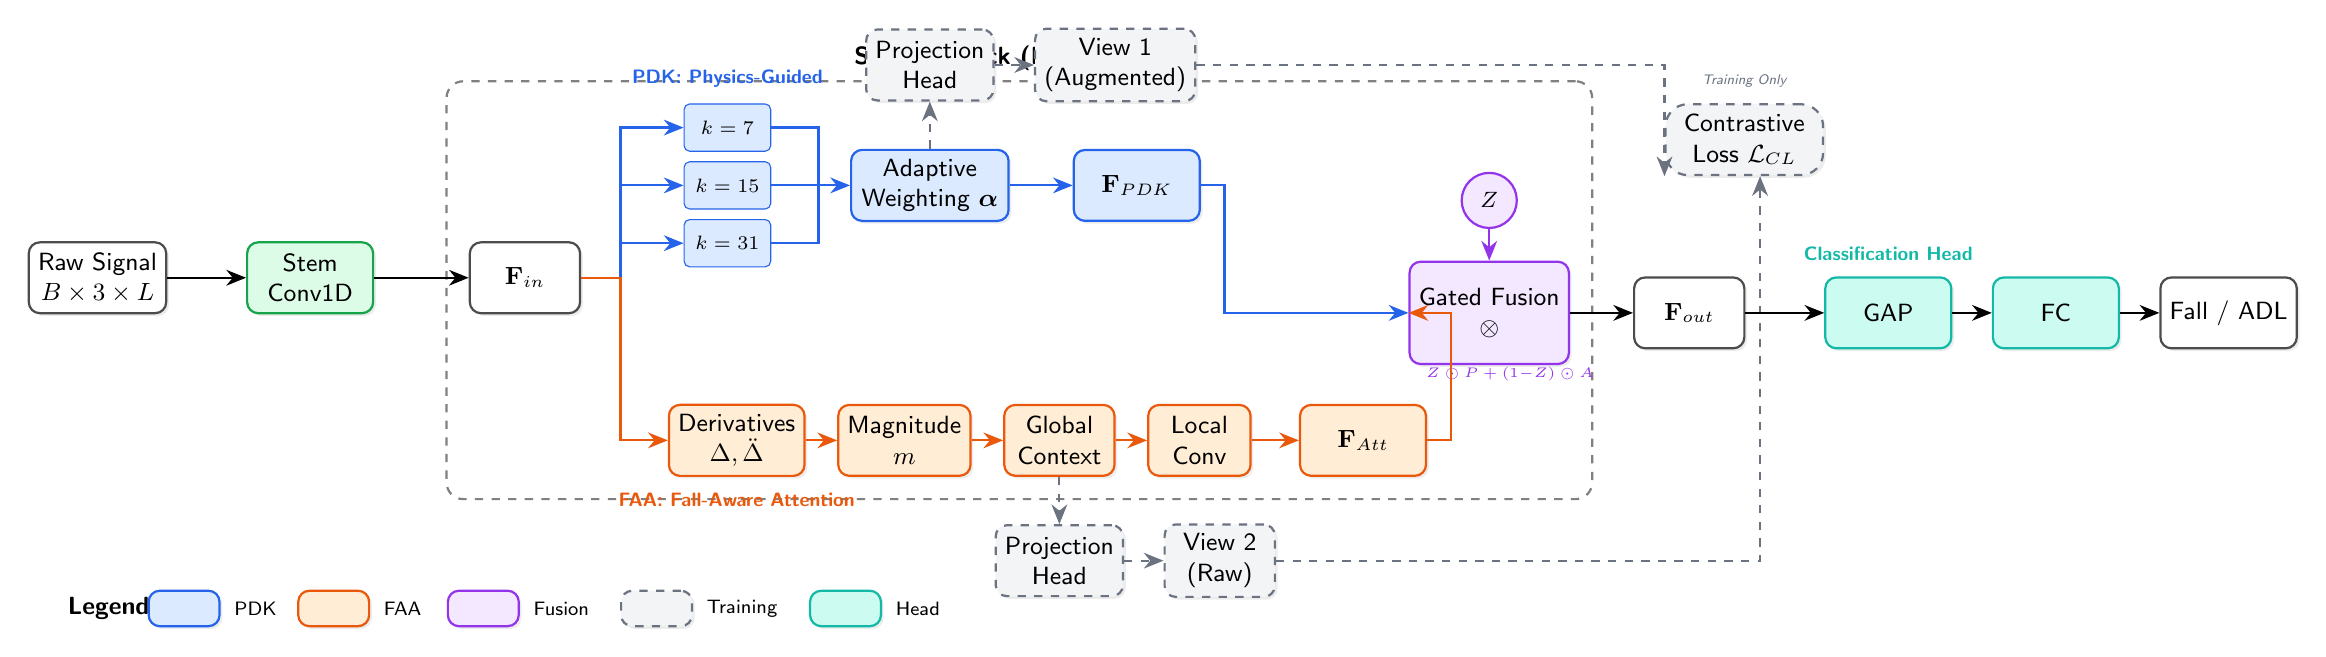
\begin{tikzpicture}[
    % ============================================
    % NODE STYLES
    % ============================================
    font=\sffamily\small,
    % Basic block
    block/.style={
        rectangle, rounded corners=4pt, 
        minimum height=0.9cm, minimum width=1.6cm,
        align=center, draw, thick,
        drop shadow={opacity=0.15, shadow xshift=1pt, shadow yshift=-1pt}
    },
    % Tensor (data)
    tensor/.style={
        block, fill=white, draw=black!70,
        minimum width=1.4cm
    },
    % Operation circle
    op/.style={
        circle, draw, thick, minimum size=0.7cm,
        fill=white, align=center, font=\sffamily\footnotesize
    },
    % PDK style
    pdk/.style={block, fill=pdkfill, draw=pdkdraw},
    % FAA style
    faa/.style={block, fill=faafill, draw=faadraw},
    % Fusion style
    fuse/.style={block, fill=fusefill, draw=fusedraw},
    % Training style
    train/.style={block, fill=trainfill, draw=traindraw, dashed},
    % Stem style
    stem/.style={block, fill=stemfill, draw=stemdraw},
    % Head style
    head/.style={block, fill=headfill, draw=headdraw},
    % Loss node
    loss/.style={
        block, fill=trainfill, draw=traindraw, dashed,
        rounded corners=8pt, minimum width=2cm
    },
    % Kernel node (small)
    kernel/.style={
        rectangle, rounded corners=2pt, 
        minimum height=0.6cm, minimum width=1.1cm,
        align=center, draw=pdkdraw, fill=pdkfill,
        font=\sffamily\scriptsize
    },
    % Arrow styles
    arr/.style={-{Stealth[length=2.5mm, width=2mm]}, thick},
    darr/.style={-{Stealth[length=2.5mm, width=2mm]}, thick, dashed, draw=traindraw},
    % Fit box style
    stagebox/.style={
        draw=black!50, dashed, rounded corners=6pt,
        inner sep=8pt, thick
    },
]

% ============================================
% CONTAINER 1: INPUT & STEM
% ============================================
\node[tensor] (input) at (0, 0) {Raw Signal\\$B \times 3 \times L$};
\node[stem, right=1cm of input] (stem) {Stem\\Conv1D};

\draw[arr] (input) -- (stem);

% ============================================
% CONTAINER 2: DUAL-BRANCH BLOCK
% ============================================

% --- Block Input ---
\node[tensor, right=1.2cm of stem] (fin) {$\mathbf{F}_{in}$};
\draw[arr] (stem) -- (fin);

% Split point
\coordinate (split) at ($(fin.east)+(0.5,0)$);

% === TOP PATH: PDK (Physics-Guided Dynamic Kernel) ===
% Multi-scale kernels - 更紧凑的布局
\node[kernel, above right=1.6cm and 0.8cm of split] (k7) {$k=7$};
\node[kernel, below=0.12cm of k7] (k15) {$k=15$};
\node[kernel, below=0.12cm of k15] (k31) {$k=31$};

% Adaptive weighting
\node[pdk, right=1cm of k15, minimum width=2cm] (alpha) {Adaptive\\Weighting $\boldsymbol{\alpha}$};

% PDK output
\node[pdk, right=0.8cm of alpha] (fpdk) {$\mathbf{F}_{PDK}$};

% PDK arrows - 简化连接
\draw[arr, draw=pdkdraw] (fin.east) -- (split) |- (k7.west);
\draw[arr, draw=pdkdraw] (split) |- (k15.west);
\draw[arr, draw=pdkdraw] (split) |- (k31.west);

% 使用更简洁的汇聚方式
\coordinate (alphaIn) at ($(alpha.west)+(-0.4,0)$);
\draw[thick, draw=pdkdraw] (k7.east) -| (alphaIn);
\draw[thick, draw=pdkdraw] (k15.east) -- (alphaIn);
\draw[thick, draw=pdkdraw] (k31.east) -| (alphaIn);
\draw[arr, draw=pdkdraw] (alphaIn) -- (alpha.west);

\draw[arr, draw=pdkdraw] (alpha) -- (fpdk);

% PDK label
\node[font=\sffamily\scriptsize\bfseries, text=pdkdraw, above=0.08cm of k7] {PDK: Physics-Guided};

% === BOTTOM PATH: FAA (Fall-Aware Attention) ===
% Derivatives & Magnitude - 调整间距
\node[faa, below right=1.6cm and 0.6cm of split, minimum width=1.5cm] (deriv) {Derivatives\\$\Delta, \ddot{\Delta}$};
\node[faa, right=0.4cm of deriv, minimum width=1.3cm] (mag) {Magnitude\\$m$};

% Global + Local
\node[faa, right=0.4cm of mag, minimum width=1.4cm] (global) {Global\\Context};
\node[faa, right=0.4cm of global, minimum width=1.3cm] (local) {Local\\Conv};

% FAA output
\node[faa, right=0.6cm of local] (fatt) {$\mathbf{F}_{Att}$};

% FAA arrows
\draw[arr, draw=faadraw] (fin.east) -- (split) |- (deriv.west);
\draw[arr, draw=faadraw] (deriv) -- (mag);
\draw[arr, draw=faadraw] (mag) -- (global);
\draw[arr, draw=faadraw] (global) -- (local);
\draw[arr, draw=faadraw] (local) -- (fatt);

% FAA label
\node[font=\sffamily\scriptsize\bfseries, text=faadraw, below=0.08cm of deriv] {FAA: Fall-Aware Attention};

% === FUSION NODE ===
% 计算融合节点位置 - 居中于两条路径之间
\coordinate (midpoint) at ($(fpdk.east)!0.5!(fatt.east)$);
\node[fuse, minimum width=2cm, minimum height=1.3cm, right=1.2cm of midpoint] (fusion) {Gated Fusion\\$\otimes$};

% Gate Z - 调整位置
\node[op, fill=fusefill, draw=fusedraw, above=0.4cm of fusion] (gatez) {$Z$};

% Fusion formula annotation
\node[font=\sffamily\tiny, text=fusedraw, below right=-0.1cm and 0.1cm of fusion.south west, anchor=north west] {$Z \odot P + (1{-}Z) \odot A$};

% Fusion arrows - 简化路径
\draw[arr, draw=pdkdraw] (fpdk.east) -- ++(0.3,0) |- (fusion.west);
\draw[arr, draw=faadraw] (fatt.east) -- ++(0.3,0) |- (fusion.west);
\draw[arr, draw=fusedraw] (gatez) -- (fusion);

% Block output
\node[tensor, right=0.8cm of fusion] (fout) {$\mathbf{F}_{out}$};
\draw[arr] (fusion) -- (fout);

% === FIT BOX: Stage Block ===
\begin{scope}[on background layer]
    \node[stagebox, fit=(k7)(k31)(alpha)(fpdk)(deriv)(local)(fatt)(fusion)(gatez)(fin), 
          label={[font=\sffamily\small\bfseries]above:Stage $i$ Block (Dual-Branch)}] (stagebox) {};
\end{scope}

% ============================================
% CONTAINER 3: TRAINING AUXILIARIES
% ============================================

% View 1 (above PDK path) - 调整位置
\node[train, above=0.6cm of alpha, minimum width=1.5cm] (proj1) {Projection\\Head};
\node[train, right=0.5cm of proj1, minimum width=1.4cm] (view1) {View 1\\(Augmented)};

% View 2 (below FAA path)
\node[train, below=0.6cm of global, minimum width=1.5cm] (proj2) {Projection\\Head};
\node[train, right=0.5cm of proj2, minimum width=1.4cm] (view2) {View 2\\(Raw)};

% Contrastive Loss - 调整位置
\node[loss, right=1.2cm of fusion, yshift=2.2cm] (closs) {Contrastive\\Loss $\mathcal{L}_{CL}$};

% Training arrows
\draw[darr] (alpha.north) -- (proj1.south);
\draw[darr] (proj1) -- (view1);
\draw[darr] (view1.east) -| (closs.south west);

\draw[darr] (global.south) -- (proj2.north);
\draw[darr] (proj2) -- (view2);
\draw[darr] (view2.east) -| ($(closs.south)+(0.2,0)$);

% Training label
\node[font=\sffamily\tiny\itshape, text=traindraw, above=0.08cm of closs] {Training Only};

% ============================================
% CONTAINER 4: OUTPUT HEAD
% ============================================

\node[head, right=1cm of fout] (gap) {GAP};
\node[head, right=0.5cm of gap] (fc) {FC};
\node[tensor, right=0.5cm of fc, minimum width=1.4cm] (output) {Fall / ADL};

\draw[arr] (fout) -- (gap);
\draw[arr] (gap) -- (fc);
\draw[arr] (fc) -- (output);

% Output head label
\node[font=\sffamily\scriptsize\bfseries, text=headdraw, above=0.08cm of gap] {Classification Head};

% ============================================
% LEGEND - 更紧凑的图例
% ============================================
\begin{scope}[shift={(-0.5, -4.2)}]
    \node[font=\sffamily\small\bfseries, anchor=west] at (0, 0) {Legend:};
    
    \node[pdk, minimum width=0.9cm, minimum height=0.45cm] (lpdk) at (1.6, 0) {};
    \node[font=\sffamily\scriptsize, right=0.05cm of lpdk] {PDK};
    
    \node[faa, minimum width=0.9cm, minimum height=0.45cm] (lfaa) at (3.5, 0) {};
    \node[font=\sffamily\scriptsize, right=0.05cm of lfaa] {FAA};
    
    \node[fuse, minimum width=0.9cm, minimum height=0.45cm] (lfuse) at (5.4, 0) {};
    \node[font=\sffamily\scriptsize, right=0.05cm of lfuse] {Fusion};
    
    \node[train, minimum width=0.9cm, minimum height=0.45cm] (ltrain) at (7.6, 0) {};
    \node[font=\sffamily\scriptsize, right=0.05cm of ltrain] {Training};
    
    \node[head, minimum width=0.9cm, minimum height=0.45cm] (lhead) at (10, 0) {};
    \node[font=\sffamily\scriptsize, right=0.05cm of lhead] {Head};
\end{scope}

\end{tikzpicture}
\end{document}
